\documentclass[11pt, oneside]{article} 
\usepackage{geometry}
\geometry{letterpaper} 
\usepackage{graphicx}
	
\usepackage{amssymb}
\usepackage{amsmath}
\usepackage{parskip}
\usepackage{color}
\usepackage{hyperref}

\graphicspath{{/Users/telliott/Github/calculus_book/png/}}
% \begin{center} 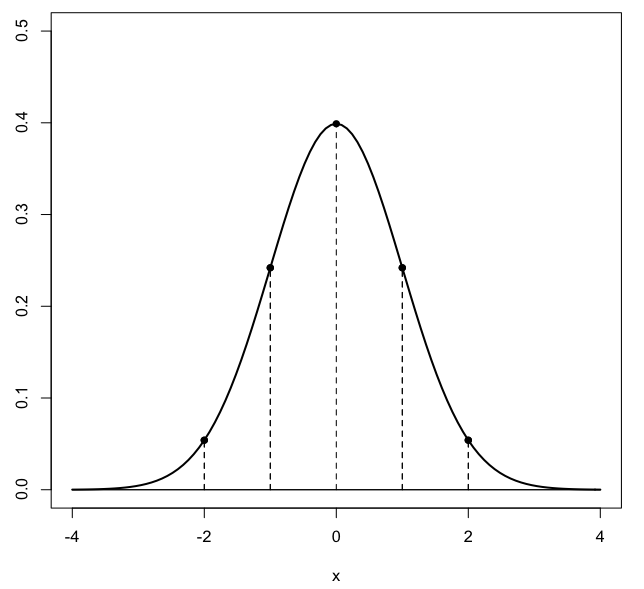
\includegraphics [scale=0.4] {gauss3.png} \end{center}

\title{Isosceles backward}
\date{}

\begin{document}
\maketitle
\Large

\label{sec:isosceles_backward}

$\circ$  The base angles of an isosceles triangle are equal.  Also, if the two base angles are equal, the triangle is isosceles.

Euclid's proof is here:

\begin{center} 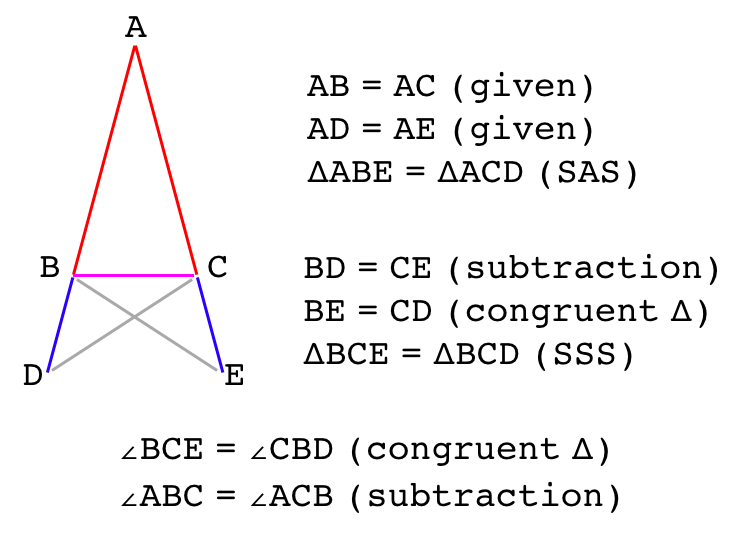
\includegraphics [scale=0.5] {isosceles_proof.png} \end{center}

Sometimes proofs can get a little complicated.  

The theorem says that the base angles are equal $\iff$ the two sides sides (not the base) are equal.  We proved that equal sides lead to equal angles, now we must proceed backwards, from equal angles to equal sides:

\begin{center} 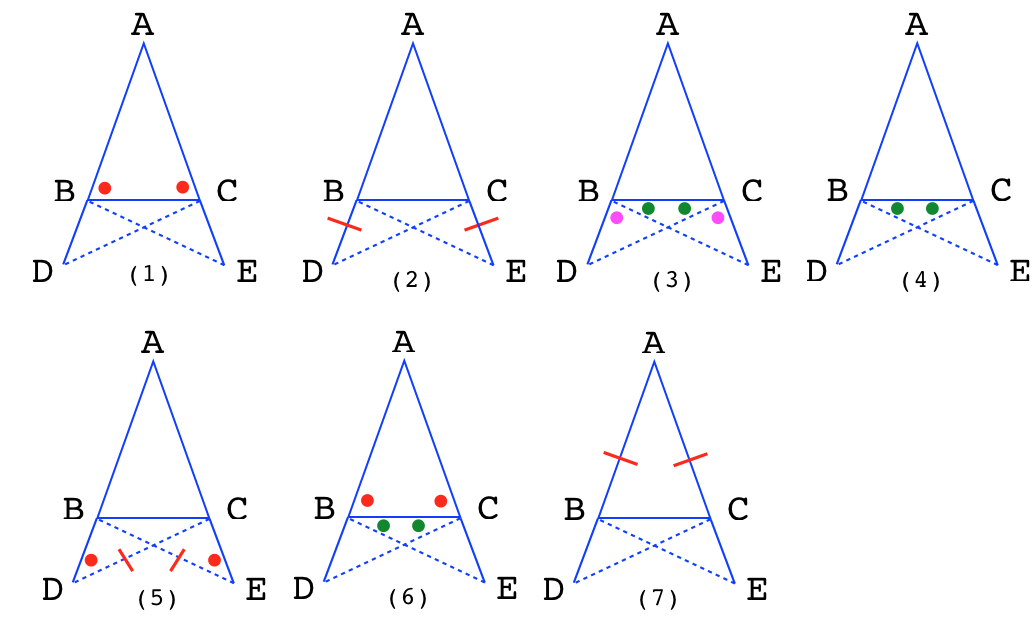
\includegraphics [scale=0.4] {isosceles5.png} \end{center}

$\circ$ \ $\angle ABC = \angle ACB$, given, (1)

$\circ$ \ $BD =CE$, by construction, (2)

$\circ$ \ $\angle DBC = \angle BCE$, supplementary angles, (3)

$\circ$ \ $\triangle DBC = \triangle BCE$, S-A-S, (3)

$\circ$ \ $\angle BCD = \angle CBE$, congruent triangles (4)

$\circ$ \ $\angle ADC = \angle AEB$, congruent triangles (5)

$\circ$ \ $BE = CD$, congruent triangles (5)

$\circ$ \ $\angle ADC = \angle ABE$, angle addition

$\circ$ \ $\triangle ADC = \triangle ABE$, A-S-A

$\circ$ \ $AB = AC$, congruent triangles

$\square$


\end{document}